\let\negmedspace\undefined
\let\negthickspace\undefined
\documentclass[journal,12pt,onecolumn]{IEEEtran}
\usepackage{cite}
\usepackage{amsmath,amssymb,amsfonts,amsthm}
\usepackage{algorithmic}
\usepackage{graphicx}
\graphicspath{{./figs/}}
\usepackage{textcomp}
\usepackage{xcolor}
\usepackage{txfonts}
\usepackage{listings}
\usepackage{enumitem}
\usepackage{mathtools}
\usepackage{gensymb}
\usepackage{comment}
\usepackage{caption}
\usepackage[breaklinks=true]{hyperref}
\usepackage{tkz-euclide} 
\usepackage{listings}
\usepackage{gvv}                                        
%\def\inputGnumericTable{}                                 
\usepackage[latin1]{inputenc}     
\usepackage{xparse}
\usepackage{color}                                            
\usepackage{array}                                            
\usepackage{longtable}                                       
\usepackage{calc}                                             
\usepackage{multirow}
\usepackage{multicol}
\usepackage{hhline}                                           
\usepackage{ifthen}                                           
\usepackage{lscape}
\usepackage{tabularx}
\usepackage{array}
\usepackage{float}
\newtheorem{theorem}{Theorem}[section]
\newtheorem{problem}{Problem}
\newtheorem{proposition}{Proposition}[section]
\newtheorem{lemma}{Lemma}[section]
\newtheorem{corollary}[theorem]{Corollary}
\newtheorem{example}{Example}[section]
\newtheorem{definition}[problem]{Definition}
\newcommand{\BEQA}{\begin{eqnarray}}
\newcommand{\EEQA}{\end{eqnarray}}
\newcommand{\define}{\stackrel{\triangle}{=}}
\theoremstyle{remark}
\newtheorem{rem}{Remark}

\begin{document}
\begin{center}
\LARGE \textbf{Assignment : GATE 2022 MA}\\[2pt] 
\large EE25BTECH11061-- Vankudoth Sainadh
\end{center}

\begin{enumerate}
   \item As you grow older, an injury to your \underline{\hspace{2cm}} may take longer to \underline{\hspace{2cm}}.

\hfill{\brak{\text{GATE MA 2022}}}

\begin{enumerate}
\begin{multicols}{2}
\item heel / heel
\item heal / heel
\item heal / heal
\item heel / heal
\end{multicols}
\end{enumerate}


\item In a $500$ m race, P and Q have speeds in the ratio $3 \colon 4$. Q starts the race when P has already covered $140$ m. What is the distance between P and Q \brak{\text{in m}} when P wins the race?

\hfill{\brak{\text{GATE MA 2022}}}

\begin{enumerate}
\begin{multicols}{2}
\item $20$
\item $40$
\item $60$
\item $140$
\end{multicols}
\end{enumerate}
\item Three bells $P$, $Q$, and $R$ are rung periodically in a school. $P$ is rung every $20$ minutes; $Q$ is rung every $30$ minutes and $R$ is rung every $50$ minutes. If all the three bells are rung at $12\colon 00$ PM, when will the three bells ring together again the next time?

\hfill{\brak{\text{GATE MA 2022}}}

\begin{enumerate}
\begin{multicols}{4}
\item $5\colon 00$ PM
\item $5\colon 30$ PM
\item $6\colon 00$ PM
\item $6\colon 30$ PM
\end{multicols}
\end{enumerate}

    
\item Given below are two statements and four conclusions drawn based on the statements.  

\begin{enumerate}

\item Statement 1: Some bottles are cups.  
\item Statement 2: All cups are knives.
\item Conclusion I: Some bottles are knives. 
\item Conclusion II: Some knives are cups.
\item Conclusion III: All cups are bottles.
\item Conclusion IV: All knives are cups. 

\end{enumerate}

Which one of the following options can be logically inferred?  

\hfill{\brak{\text{GATE MA 2022}}}

\begin{enumerate}

\item Only conclusion I and conclusion II are correct  
\item Only conclusion II and conclusion III are correct  
\item Only conclusion II and conclusion IV are correct  
\item Only conclusion III and conclusion IV are correct  

\end{enumerate}
\item The figure below shows the front and rear view of a disc, which is shaded with identical patterns. The disc is flipped once with respect to any one of the fixed axes \brak{\text{1-1, 2-2 or 3-3}} chosen uniformly at random. What is the probability that the disc DOES NOT retain the same front and rear views after the flipping operation?

\hfill{\brak{\text{GATE MA 2022}}}

\begin{figure}[h!]
\centering
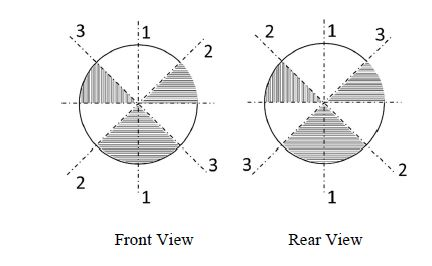
\includegraphics[width = 0.85\columnwidth]{figs/q5.png}
\caption{*}
\label{fig:placeholder}
\end{figure}

\begin{enumerate}
\begin{multicols}{4}

\item $0$
\item $\frac{1}{3}$
\item $\frac{2}{3}$
\item $1$
\end{multicols}
\end{enumerate}

\item Altruism is the human concern for the wellbeing of others. Altruism has been shown to be motivated more by social bonding, familiarity and identification of belongingness to a group. The notion that altruism may be attributed to empathy or guilt has now been rejected. Which one of the following is the CORRECT logical inference based on the information in the above passage?

\hfill{\brak{\text{GATE MA 2022}}}

\begin{enumerate}
\item Humans engage in altruism due to guilt but not empathy
\item Humans engage in altruism due to empathy but not guilt
\item Humans engage in altruism due to group identification but not empathy
\item Humans engage in altruism due to empathy but not familiarity
\end{enumerate}
\item There are two identical dice with a single letter on each of the faces. The following six letters: Q, R, S, T, U, and V, one on each of the faces. Any of the six outcomes are equally likely. The two dice are thrown once independently at random. What is the probability that the outcomes on the dice were composed only of any combination of the following possible outcomes$\colon$ Q, U and V? 

\hfill{\brak{\text{GATE MA 2022}}}

\begin{enumerate}
\begin{multicols}{4}

\item $\dfrac{1}{4}$  
\item $\dfrac{3}{4}$  
\item $\dfrac{1}{6}$  
\item $\dfrac{5}{36}$  

\end{multicols}
\end{enumerate}


\item The price of an item is $10\%$ cheaper in an online store S compared to the price at another online store M. Store S charges  $150$ for delivery. There are no delivery charges for orders from the store M. A person bought the item from the store S and saved  $100$. What is the price of the item at the online store S \brak{\text{in rupees}} if there are no other charges than what is described above?

\hfill{\brak{\text{GATE MA 2022}}}

\begin{enumerate}
\begin{multicols}{4}
  \item $2500$
\item $2250$
\item $1750$
\item $1500$
  
\end{multicols}
\end{enumerate}

\item The letters P, Q, R, S, T and U are to be placed one per vertex on a regular convex hexagon, but not necessarily in the same order.  

Consider the following statements$\colon$
\begin{itemize}
\item The line segment joining R and S is longer than the line segment joining P and Q.  
\item The line segment joining R and S is perpendicular to the line segment joining P and Q.  
\item The line segment joining R and U is parallel to the line segment joining T and Q.  \end{itemize}

Based on the above statements, which one of the following options is CORRECT?

\hfill{\brak{\text{GATE MA 2022}}}

\begin{enumerate}
\item The line segment joining R and T is parallel to the line segment joining Q and S.
\item The line segment joining T and Q is parallel to the line joining P and U.
\item The line segment joining R and P is perpendicular to the line segment joining U and Q.
\item The line segment joining Q and S is perpendicular to the line segment joining R and P.
\end{enumerate}

\item An ant is at the bottom-left corner of a grid \brak{\text{point } P} as shown below. It aims to move to the top-right corner of the grid. The ant moves only along the lines marked in the grid such that the current distance to the top-right corner strictly decreases. Which one of the following is a part of a possible trajectory of the ant during the movement?

\hfill{\brak{\text{GATE MA 2022}}}


\begin{figure}[h!]
\centering
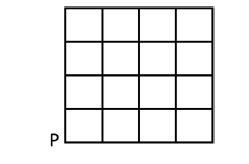
\includegraphics[width = 0.4\columnwidth]{figs/q10.png}
\caption{*}
\label{fig:placeholder}
\end{figure}

\begin{multicols}{2}
\begin{enumerate}

\item 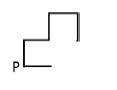
\includegraphics[width=0.4\columnwidth]{figs/a38a.png}
\item 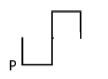
\includegraphics[width=0.4\columnwidth]{figs/a38b.png}
\item 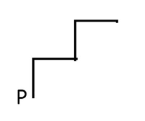
\includegraphics[width=0.4\columnwidth]{figs/a38c.png}
\item 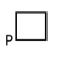
\includegraphics[width=0.4\columnwidth]{figs/a38d.png}
\end{enumerate}
\end{multicols}

\item Suppose that the characteristic equation of $M \in \mathbb{C}^{3\times 3}$ is $\lambda^{3} + \alpha \lambda^{2} + \beta \lambda - 1 = 0$, where $\alpha, \beta \in \mathbb{C}$ with $\alpha + \beta \ne 0$. Which of the following statements is TRUE?

\hfill{\brak{\text{GATE MA 2022}}}


\begin{enumerate}
\begin{multicols}{2}
  \item $M\brak{I - \beta M} = M^{-1}\brak{M + \alpha I}$
\item $M\brak{I + \beta M} = M^{-1}\brak{M - \alpha I}$
\item $M^{-1}\brak{M^{-1} + \beta I} = M - \alpha I$
\item $M^{-1}\brak{M^{-1} - \beta I} = M + \alpha I$
  
\end{multicols}
\end{enumerate}
\newpage
\item Consider

$P$ $\colon$ Let $M \in \mathbb{R}^{m\times n}$ with $m>n\ge 2$. If $\operatorname{rank}\brak{M}=n$, then the system of linear equations $Mx=0$ has $x=0$ as the only solution.

$Q$ $\colon$ Let $E \in \mathbb{R}^{n\times n}$, $n\ge 2$ be a non-zero matrix such that $E^{3}=0$. Then $I+E^{2}$ is a singular matrix.

Which of the following statements is TRUE?

\hfill{\brak{\text{GATE MA 2022}}}

\begin{enumerate}
\item Both $P$ and $Q$ are TRUE
\item Both $P$ and $Q$ are FALSE
\item $P$ is TRUE and $Q$ is FALSE
\item $P$ is FALSE and $Q$ is TRUE
\end{enumerate}

\item Consider the real function of two real variables given by
$$u\brak{x,y} = e^{2x}\brak{\sin 3x \cos 2y \cosh 3y - \cos 3x \sin 2y \sinh 3y}.$$\\
Let $v\brak{x,y}$ be the harmonic conjugate of $u\brak{x,y}$ such that $v\brak{0,0}=2$. Let $z=x+iy$ and $f\brak{z}=u\brak{x,y}+i\,v\brak{x,y}$, then the value of $4+2i\,f\brak{i\pi}$ is

\hfill{\brak{\text{GATE MA 2022}}}

\begin{enumerate}
\begin{multicols}{2}
  \item $e^{3\pi}+e^{-3\pi}$
\item $e^{3\pi}-e^{-3\pi}$
\item $-e^{3\pi}+e^{-3\pi}$
\item $-e^{3\pi}-e^{-3\pi}$
\end{multicols}
\end{enumerate}

\item The value of the integral
\begin{align*}
\int_{C} \frac{z^{100}}{z^{101}+1}\,dz
\end{align*}
where $C$ is the circle of radius $2$ centred at the origin taken in the anti-clockwise direction, is

\hfill{\brak{\text{GATE MA 2022}}}

\begin{enumerate}
\begin{multicols}{4}
\item $-2\pi i$
\item $2\pi$
\item $0$
\item $2\pi i$
  
\end{multicols}
\end{enumerate}

\item Let $X$ be a real normed linear space. Let $X_{0} = \{x \in X \colon \lVert x \rVert = 1\}$. If $X_{0}$ contains two distinct points $x$ and $y$ and the line segment joining them, which of the following statements is TRUE?

\hfill{\brak{\text{GATE MA 2022}}}

\begin{enumerate}
\item $\lVert x + y \rVert = \lVert x \rVert + \lVert y \rVert$ and $x, y$ are linearly independent
\item $\lVert x + y \rVert = \lVert x \rVert + \lVert y \rVert$ and $x, y$ are linearly dependent
\item $\lVert x + y \rVert^{2} = \lVert x \rVert^{2} + \lVert y \rVert^{2}$ and $x, y$ are linearly independent
\item $\lVert x + y \rVert = 2 \lVert x \rVert \lVert y \rVert$ and $x, y$ are linearly dependent
\end{enumerate}

\item Let $\{e_{k} \colon k \in \mathbb{N}\}$ be an orthonormal basis for a Hilbert space $H$. Define $f_{k}=e_{k}+e_{k+1}$ for $k \in \mathbb{N}$ and $g_{j}=\displaystyle\sum\limits_{n=1}^{j}\brak{-1}^{\,n+1}e_{n}$ for $j \in \mathbb{N}$. Then

\begin{align*}
\sum\limits_{k=1}^{\infty}\abs{\langle g_{j},f_{k}\rangle}^{2}= 
\end{align*}

\hfill{\brak{\text{GATE MA 2022}}}

\begin{enumerate}
\begin{multicols}{4}
\item $0$
\item $j^{2}$
\item $4j^{2}$
\item $1$
 
\end{multicols}
\end{enumerate}



\newpage
\item Consider $\mathbb{R}^{2}$ with the usual metric. Let
$A=\{\brak{x,y}\in \mathbb{R}^{2}\colon x^{2}+y^{2}\le 1\}$ and
$B=\{\brak{x,y}\in \mathbb{R}^{2}\colon \brak{x-2}^{2}+y^{2}\le 1\}$.
Let $M=A\cup B$ and $N=\operatorname{interior}\brak{A}\cup \operatorname{interior}\brak{B}$.
Then, which of the following statements is TRUE?

\hfill{\brak{\text{GATE MA 2022}}}

\begin{enumerate}
\item $M$ and $N$ are connected
\item Neither $M$ nor $N$ is connected
\item $M$ is connected and $N$ is not connected
\item $M$ is not connected and $N$ is connected
\end{enumerate}


\item The real sequence generated by the iterative scheme
\begin{align*}
x_{n} = \frac{x_{n-1}}{2} + \frac{1}{x_{n-1}}, \quad n \ge 1
\end{align*}

\hfill{\brak{\text{GATE MA 2022}}}

\begin{enumerate}
\item converges to $\sqrt{2}$, for all $x_{0} \in \mathbb{R} \setminus \{0\}$
\item converges to $\sqrt{2}$, whenever $x_{0} > \sqrt{\tfrac{2}{3}}$
\item converges to $\sqrt{2}$, whenever $x_{0} \in \brak{-1, 1} \setminus \{0\}$
\item diverges for any $x_{0} \ne 0$
\end{enumerate}

\item The initial value problem
\begin{align*}
\frac{dy}{dx} &= \cos\brak{xy}, \quad x \in \mathbb{R}, \quad y\brak{0} = y_0,
\end{align*}
where $y_0$ is a real constant, has

\hfill{\brak{\text{GATE MA 2022}}}

\begin{enumerate}
\begin{multicols}{2}
\item a unique solution
\item exactly two solutions
\item infinitely many solutions
\item no solution
\end{multicols}
\end{enumerate}

\item If eigenfunctions corresponding to distinct eigenvalues $\lambda$ of the Sturm--Liouville problem
\begin{align*}
\frac{d^{2}y}{dx^{2}} - 3\,\frac{dy}{dx} &= \lambda y,\quad 0 < x < \pi,\\
y\brak{0} &= y\brak{\pi} = 0
\end{align*}
are orthogonal with respect to the weight function $w\brak{x}$, then $w\brak{x}$ is

\hfill{\brak{\text{GATE MA 2022}}}

\begin{enumerate}
\begin{multicols}{4}
\item $e^{-3x}$
\item $e^{-2x}$
\item $e^{2x}$
\item $e^{3x}$
\end{multicols}
\end{enumerate}

\item The steady state solution for the heat equation
\begin{align*}
\frac{\partial u}{\partial t} - \frac{\partial^{2} u}{\partial x^{2}} = 0,\quad \brak{0 < x < 2,\, t > 0},
\end{align*}
with the initial condition $u\brak{x,0}=0$, $\brak{0 < x < 2}$ and the boundary conditions $u\brak{0,t}=1$ and $u\brak{2,t}=3$, $t>0$, at $x=1$ is

\hfill{\brak{\text{GATE MA 2022}}}

\begin{enumerate}
\begin{multicols}{4}
\item $1$
\item $2$
\item $3$
\item $4$
\end{multicols}
\end{enumerate}
\newpage
\item Consider $\brak{[0,1], T_{1}}$, where $T_{1}$ is the subspace topology induced by the Euclidean topology on $\mathbb{R}$, and let $T_{2}$ be any topology on $[0,1]$. Consider the following statements.

P $\colon$ If $T_{1}$ is a proper subset of $T_{2}$, then $\brak{[0,1], T_{2}}$ is not compact.

Q $\colon$ If $T_{2}$ is a proper subset of $T_{1}$, then $\brak{[0,1], T_{2}}$ is not Hausdorff.

Then

\hfill{\brak{\text{GATE MA 2022}}}

\begin{enumerate}
\item P is TRUE and Q is FALSE
\item Both P and Q are TRUE
\item Both P and Q are FALSE
\item P is FALSE and Q is TRUE
\end{enumerate}

\item Let $p \colon \brak{[0,1], T_{1}} \to \brak{\{0,1\}, T_{2}}$ be the quotient map arising from the characteristic function on $\left[\tfrac{1}{2}, 1\right]$, where $T_{1}$ is the subspace topology induced by the Euclidean topology on $\mathbb{R}$. Which of the following statements is TRUE?

\hfill{\brak{\text{GATE MA 2022}}}

\begin{enumerate}
\item $p$ is an open map but not a closed map
\item $p$ is a closed map but not an open map
\item $p$ is a closed map as well as an open map
\item $p$ is neither an open map nor a closed map
\end{enumerate}

\item Set $X_{n} := \mathbb{R}$ for each $n \in \mathbb{N}$. Define $Y := \displaystyle\prod_{n\in\mathbb{N}} X_{n}$. Endow $Y$ with the product topology, where the topology on each $X_{n}$ is the Euclidean topology. Consider the set
\begin{align*}
\Delta = \left\{\brak{x, x, x, \cdots} \mid x \in \mathbb{R}\right\}
\end{align*}
with the subspace topology induced from $Y$. Which of the following statements is TRUE?

\hfill{\brak{\text{GATE MA 2022}}}

\begin{enumerate}
\begin{multicols}{2}
 \item $\Delta$ is open in $Y$
\item $\Delta$ is locally compact
\item $\Delta$ is dense in $Y$
\item $\Delta$ is disconnected
   
\end{multicols}
\end{enumerate}

\item Consider the linear system of equations $Ax=b$ with
\begin{align*}
A &= \myvec{3 & 1 & 1 \\ 1 & 4 & 1 \\ 2 & 0 & 3}, \quad
b = \myvec{2 \\ 3 \\ 4}.
\end{align*}
Which of the following statements are TRUE?

\hfill{\brak{\text{GATE MA 2022}}}

\begin{enumerate}
\item The Jacobi iterative matrix is ~$\myvec{0 & \tfrac{1}{4} & \tfrac{1}{3} \\[4pt]
\tfrac{1}{3} & 0 & \tfrac{1}{3} \\[4pt]
\tfrac{2}{3} & 0 & 0}$

\item The Jacobi iterative method converges for any initial vector
\item The Gauss\textendash Seidel iterative method converges for any initial vector
\item The spectral radius of the Jacobi iterative matrix is less than $1$
\end{enumerate}

\item The number of non-isomorphic abelian groups of order $2^{2}\cdot 3^{3}\cdot 5^{4}$ is \underline{\hspace{2cm}}.

\hfill{\brak{\text{GATE MA 2022}}}

\item The number of subgroups of a cyclic group of order $12$ is \underline{\hspace{2cm}}.

\hfill{\brak{\text{GATE MA 2022}}}
\newpage
\item The radius of convergence of the series
\begin{align*}
\sum_{n\ge 0} 3^{n+1} z^{2n}, \quad z\in \mathbb{C}
\end{align*}
is \brak{\text{round off to TWO decimal places}} \underline{\hspace{2cm}}.

\hfill{\brak{\text{GATE MA 2022}}}

\item The number of zeros of the polynomial ~$2z^{7} - 7z^{5} + 2z^{3} - z + 1$ in the unit disc $\{z \in \mathbb{C} \colon \abs{z} < 1\}$ is \underline{\hspace{2cm}}.

\hfill{\brak{\text{GATE MA 2022}}}

\item If $P\brak{x}$ is a polynomial of degree $5$ and
\begin{align*}
\alpha \;=\; \sum_{i=0}^{6} P\brak{x_{i}} \,\brak{\prod_{\substack{j=0 \\ j\ne i}}^{6} \brak{x_{i}-x_{j}}^{-1}},
\end{align*}
where $x_{0}, x_{1}, \dots, x_{6}$ are distinct points in the interval $[2,3]$, then the value of $\alpha^{2}-\alpha+1$ is \underline{\hspace{2cm}}.

\hfill{\brak{\text{GATE MA 2022}}}

\item The maximum value of $f\brak{x,y} = 49 - x^{2} - y^{2}$ on the line $x + 3y = 10$ is \underline{\hspace{2cm}}.

\hfill{\brak{\text{GATE MA 2022}}}

\item If the function $f\brak{x,y} = x^{2} + xy + y^{2} + \dfrac{1}{x} + \dfrac{1}{y}$ for $x \ne 0$, $y \ne 0$ attains its local minimum value at the point $\brak{a,b}$, then the value of $a^{3}+b^{3}$ is \brak{\text{round off to TWO decimal places}} \underline{\hspace{2cm}}.

\hfill{\brak{\text{GATE MA 2022}}}

\item If the ordinary differential equation
\begin{align*}
x^{2}\,\frac{d^{2}\phi}{dx^{2}} + x\,\frac{d\phi}{dx} + x^{2}\,\phi = 0,\quad x>0
\end{align*}
has a solution of the form $\phi\brak{x} = x^{r}\displaystyle\sum_{n=0}^{\infty} a_{n}x^{n}$, where $a_{n}$ are constants and $a_{0}\ne 0$, then the value of $r^{2}+1$ is \underline{\hspace{2cm}}.

\hfill{\brak{\text{GATE MA 2022}}}

\item The Bessel functions $J_{\alpha}\brak{x}$ for $x>0$, $\alpha \in \mathbb{R}$ satisfy
$J_{\alpha-1}\brak{x} + J_{\alpha+1}\brak{x} \;=\; \frac{2\alpha}{x}\,J_{\alpha}\brak{x}.$
Then, the value of $\brak{\pi\,J_{3/2}\brak{\pi}}^{2}$ is \underline{\hspace{2cm}}.

\hfill{\brak{\text{GATE MA 2022}}}

\item The partial differential equation
\begin{align*}
7\,\frac{\partial^{2}u}{\partial x^{2}}
\;+\;16\,\frac{\partial^{2}u}{\partial x\,\partial y}
\;+\;4\,\frac{\partial^{2}u}{\partial y^{2}}
\;=\;0
\end{align*}
is transformed to
\begin{align*}
A\,\frac{\partial^{2}u}{\partial \xi^{2}}
\;+\;B\,\frac{\partial^{2}u}{\partial \xi\,\partial \eta}
\;+\;C\,\frac{\partial^{2}u}{\partial \eta^{2}}
\;=\;0,
\end{align*}
using $\xi = y - 2x$ and $\eta = 7y - 2x$. Then, the value of $\dfrac{1}{123}\,\brak{B^{2}-4AC}$ is \underline{\hspace{2cm}}.

\hfill{\brak{\text{GATE MA 2022}}}
\newpage
\item Let $\mathbb{R}[X]$ denote the ring of polynomials in $X$ with real coefficients. Then, the quotient ring $\mathbb{R}[X]/\brak{X^{4} + 4}$ is

\hfill{\brak{\text{GATE MA 2022}}}

\begin{enumerate}
\item a field
\item an integral domain, but not a field
\item not an integral domain, but has $0$ as the only nilpotent element
\item a ring which contains non\textendash zero nilpotent elements
\end{enumerate}

\item Consider the following conditions on two proper non\textendash zero ideals $J_{1}$ and $J_{2}$ of a non\textendash zero commutative ring $R$.

$P$ $\colon$ For any $r_{1}, r_{2} \in R$, there exists a unique $r \in R$ such that $r - r_{1} \in J_{1}$ and $r - r_{2} \in J_{2}$.

$Q$ $\colon$ $J_{1} + J_{2} = R$.

Then, which of the following statements is TRUE?

\hfill{\brak{\text{GATE MA 2022}}}

\begin{enumerate}
\item $P$ implies $Q$ but $Q$ does not imply $P$
\item $Q$ implies $P$ but $P$ does not imply $Q$
\item $P$ implies $Q$ and $Q$ implies $P$
\item $P$ does not imply $Q$ and $Q$ does not imply $P$
\end{enumerate}

\item Let $f \colon \left[-\pi,\pi\right] \to \mathbb{R}$ be a continuous function such that $f\brak{x} > \dfrac{f\brak{0}}{2}$ for $\abs{x} < \delta$, where $0 < \delta < \pi$. Define $P_{n,\delta}\brak{x} \;=\; \brak{1 + \cos x - \cos \delta}^{n}, \quad \text{for } n = 1,2,3,\dots$
Then, which of the following statements is TRUE?

\hfill{\brak{\text{GATE MA 2022}}}

\begin{enumerate}
\begin{multicols}{2}
  \item $\displaystyle \lim_{n \to \infty} \int_{0}^{2\delta} f\brak{x}\, P_{n,\delta}\brak{x}\, dx = 0$
\item $\displaystyle \lim_{n \to \infty} \int_{-2\delta}^{0} f\brak{x}\, P_{n,\delta}\brak{x}\, dx = 0$
\item $\displaystyle \lim_{n \to \infty} \int_{-\delta}^{\delta} f\brak{x}\, P_{n,\delta}\brak{x}\, dx = 0$
\item $\displaystyle \lim_{n \to \infty} \int_{\left[-\pi,\pi\right] \setminus \left[-\delta,\delta\right]} f\brak{x}\, P_{n,\delta}\brak{x}\, dx = 0$
  
\end{multicols}
\end{enumerate}

\item $P$ $\colon$ Suppose that $\displaystyle\sum_{n=0}^{\infty} a_{n}x^{n}$ converges at $x=-3$ and diverges at $x=6$. Then $\displaystyle\sum_{n=0}^{\infty} \brak{-1}^{n} a_{n}$ converges.

$Q$ $\colon$ The interval of convergence of the series $\displaystyle\sum_{n=2}^{\infty} \frac{\brak{-1}^{n} x^{n}}{4^{n}\,\ln n}$ is $[-4,4]$.

Which of the following statements is TRUE?

\hfill{\brak{\text{GATE MA 2022}}}

\begin{enumerate}
\item $P$ is TRUE and $Q$ is TRUE
\item $P$ is FALSE and $Q$ is FALSE
\item $P$ is TRUE and $Q$ is FALSE
\item $P$ is FALSE and $Q$ is TRUE
\end{enumerate}

\item Let
\begin{align*}
f_{n}\brak{x} \;=\; \frac{x^{2}}{x^{2} + \brak{1 - n x}^{2}}, \quad x \in [0,1],\; n = 1,2,3,\dots
\end{align*}
Then, which of the following statements is TRUE?

\hfill{\brak{\text{GATE MA 2022}}}

\begin{enumerate}
\item $\{f_{n}\}$ is not equicontinuous on $[0,1]$
\item $\{f_{n}\}$ is uniformly convergent on $[0,1]$
\item $\{f_{n}\}$ is equicontinuous on $[0,1]$
\item $\{f_{n}\}$ is uniformly bounded and has a subsequence converging uniformly on $[0,1]$
\end{enumerate}
\newpage
\item Let $\brak{\mathbb{Q}, d}$ be the metric space with $d\brak{x, y} = \abs{x - y}$. Let $E = \{\, p \in \mathbb{Q} \colon 2 < p^{2} < 3 \,\}$. Then, the set $E$ is

\hfill{\brak{\text{GATE MA 2022}}}

\begin{enumerate}
\begin{multicols}{2}
\item closed but not compact
\item not closed but compact
\item compact
\item neither closed nor compact
\end{multicols}
\end{enumerate}

\item Let $T \colon \mathrm{L}^{2}{[-1,1]} \to \mathrm{L}^{2}{[-1,1]}$ be defined by $Tf=\tilde{f}$, where $\tilde{f}\brak{x}=f\brak{-x}$ \brak{\text{a.e.}} If $M$ is the kernel of $I-T$, then the distance between the function $\phi\brak{t}=e^{t}$ and $M$ is

\hfill{\brak{\text{GATE MA 2022}}}

\begin{enumerate}
\begin{multicols}{2}
\item $\dfrac{1}{2}\sqrt{e^{2}-e^{-2}+4}$
\item $\dfrac{1}{2}\sqrt{e^{2}-e^{-2}-2}$
\item $\dfrac{1}{2}\sqrt{e^{2}-4}$
\item $\dfrac{1}{2}\sqrt{e^{2}-e^{-2}-4}$
\end{multicols}
\end{enumerate}

\item Let $X$, $Y$ and $Z$ be Banach spaces. Suppose that $T \colon X \to Y$ is linear and $S \colon Y \to Z$ is linear, bounded and injective. In addition, if $S \circ T \colon X \to Z$ is bounded, then which of the following statements is TRUE?

\hfill{\brak{\text{GATE MA 2022}}}

\begin{enumerate}
\begin{multicols}{2}
\item $T$ is surjective
\item $T$ is bounded but not continuous
\item $T$ is bounded
\item $T$ is not bounded
    
\end{multicols}
\end{enumerate}

\item The first derivative of a function $f \in \mathrm{C}^{\infty}\brak{-3,3}$ is approximated by an interpolating polynomial of degree $2$, using the data $\brak{-1, f\brak{-1}}, \brak{0, f\brak{0}} \text{ and } \brak{2, f\brak{2}}$. It is found that
\begin{align*}
f'\brak{0} \approx -\frac{2}{3}\,f\brak{-1} + \alpha\,f\brak{0} + \beta\,f\brak{2}.
\end{align*}
Then, the value of $\dfrac{1}{\alpha\beta}$ is

\hfill{\brak{\text{GATE MA 2022}}}

\begin{enumerate}
\begin{multicols}{4}
\item $3$
\item $6$
\item $9$
\item $12$
\end{multicols}
\end{enumerate}

\item The work done by the force
\begin{align*}
\vec{F} \;=\; \brak{x + y}\,\hat{\imath} \;-\; \brak{x^{2} + y^{2}}\,\hat{\jmath},
\end{align*}
where $\hat{\imath}$ and $\hat{\jmath}$ are unit vectors along the $\overrightarrow{OX}$ and $\overrightarrow{OY}$ directions, respectively along the upper half of the circle $x^{2} + y^{2} = 1$ from $\brak{1,0}$ to $\brak{-1,0}$ in the $xy$-plane is

\hfill{\brak{\text{GATE MA 2022}}}

\begin{enumerate}
\begin{multicols}{4}
\item $-\pi$
\item $-\tfrac{\pi}{2}$
\item $\tfrac{\pi}{2}$
\item $\pi$
\end{multicols}
\end{enumerate}
\newpage
\item Let $u\brak{x,t}$ be the solution of the wave equation
\begin{align*}
\frac{\partial^{2}u}{\partial t^{2}} \;-\; \frac{\partial^{2}u}{\partial x^{2}} \;=\; 0,\qquad 0 < x < \pi,\; t>0,
\end{align*}
with the initial conditions
\begin{align*}
u\brak{x,0} \;=\; \sin x \;+\; \sin 2x \;+\; \sin 3x,\qquad
\frac{\partial u}{\partial t}\brak{x,0} \;=\; 0,\quad 0 < x < \pi,
\end{align*}
and the boundary conditions $u\brak{0,t} \;=\; u\brak{\pi,t} \;=\; 0,\; t \ge 0$. Then, the value of $u\brak{\tfrac{\pi}{2}, \pi}$ is

\hfill{\brak{\text{GATE MA 2022}}}


\begin{enumerate}
\begin{multicols}{4}
\item $-\dfrac{1}{2}$
\item $0$
\item $\dfrac{1}{2}$
\item $1$
\end{multicols}
\end{enumerate}

\item Let $T \colon \mathbb{R}^{2} \to \mathbb{R}^{2}$ be a linear transformation defined by
\begin{align*}
T\brak{\brak{1,2}} = \brak{1,0} \quad \text{and} \quad T\brak{\brak{2,1}} = \brak{1,1}.
\end{align*}
For $p,q \in \mathbb{R}$, let $T^{-1}\brak{\brak{p,q}} = \brak{x,y}$. Which of the following statements is TRUE?

\hfill{\brak{\text{GATE MA 2022}}}

\begin{enumerate}
\begin{multicols}{2}
\item $x = p - q;\ y = 2p - q$
\item $x = p + q;\ y = 2p - q$
\item $x = p + q;\ y = 2p + q$
\item $x = p - q;\ y = 2p + q$
\end{multicols}
\end{enumerate}

\item Let $y = \myvec{\alpha,-1}^{T}$, $\alpha \in \mathbb{R}$ be a feasible solution for the dual problem of the linear programming problem
\begin{align*}
\text{Maximize }:~ &5x_{1} + 12x_{2} \\
\text{subject to} : 
~&x_{1} + 2x_{2} + x_{3} \le 10, \\
& 2x_{1} - x_{2} + 3x_{3} = 8, \\
& x_{1}, x_{2}, x_{3} \ge 0.
\end{align*}
Which of the following statements is TRUE?

\hfill{\brak{\text{GATE MA 2022}}}

\begin{enumerate}
\begin{multicols}{4}
\item $\alpha < 3$
\item $3 \le \alpha < 5.5$
\item $5.5 \le \alpha < 7$
\item $\alpha \ge 7$
\end{multicols}
\end{enumerate}

\item Let $K$ denote the subset of $\mathbb{C}$ consisting of elements algebraic over $\mathbb{Q}$. Then, which of the following statements are TRUE?

\hfill{\brak{\text{GATE MA 2022}}}

\begin{enumerate}
\item \text{No element of } $\mathbb{C}\setminus K$ \text{ is algebraic over } $\mathbb{Q}$
\item $K$ \text{ is an algebraically closed field}
\item \text{For any bijective ring homomorphism } $f \colon \mathbb{C} \to \mathbb{C}$\text{, we have } $f\brak{K} = K$
\item \text{There is no bijection between } $K$ \text{ and } $\mathbb{Q}$
\end{enumerate}

\item Let $T$ be a Möbius transformation such that $T\brak{0} = \alpha$, $T\brak{\alpha} = 0$ and $T\brak{\infty} = -\alpha$, where $\alpha = \frac{-1 + i}{\sqrt{2}}$. Let $L$ denote the straight line passing through the origin with slope $-1$, and let $C$ denote the circle of unit radius centred at the origin. Then, which of the following statements are TRUE?

\hfill{\brak{\text{GATE MA 2022}}}

\begin{enumerate}
\item $T$ maps $L$ to a straight line
\item $T$ maps $L$ to a circle
\item $T^{-1}$ maps $C$ to a straight line
\item $T^{-1}$ maps $C$ to a circle
\end{enumerate}
\newpage
\item Let $a>0$. Define $D_a \colon L_2\brak{\mathbb{R}} \to L_2\brak{\mathbb{R}}$ by $\brak{D_a f}\brak{x} = \frac{1}{\sqrt{a}}\,f\brak{\frac{x}{a}}$, almost everywhere, for $f \in L_2\brak{\mathbb{R}}$. Then, which of the following statements are TRUE?

\hfill{\brak{\text{GATE MA 2022}}}

\begin{enumerate}
\begin{multicols}{2}
\item $D_a$ is a linear isometry
\item $D_a$ is a bijection
\item $D_a \circ D_b = D_{a+b}$, $b>0$
\item $D_a$ is bounded from below
  
\end{multicols}
\end{enumerate}

\item Let $\{\phi_0,\ \phi_1,\ \phi_2,\ \dots\}$ be an orthonormal set in $L^2[-1,1]$ such that $\phi_n = C_n P_n$, where $C_n$ is a constant and $P_n$ is the Legendre polynomial of degree $n$, for each $n\in \mathbb{N}\cup\{0\}$. Then, which of the following statements are TRUE?

\hfill{\brak{\text{GATE MA 2022}}}

\begin{enumerate}
\begin{multicols}{4}
 \item $\phi_6\brak{1} = 1$
\item $\phi_7\brak{-1} = 1$
\item $\phi_7\brak{1} = \dfrac{\sqrt{15}}{2}$
\item $\phi_6\brak{-1} = \dfrac{\sqrt{13}}{2}$   
\end{multicols}
\end{enumerate}

\item Let $X=\brak{\mathbb{R},{T}}$, where ${T}$ is the smallest topology on $\mathbb{R}$ in which all the singleton sets are closed. Then, which of the following statements are TRUE$?$ 

\hfill{\brak{\text{GATE MA 2022}}}

\begin{enumerate}
\item $\{x\in\mathbb{R}\mid 0\le x<1\}$ is compact in $X$.
\item $X$ is not first countable.
\item $X$ is second countable.
\item $X$ is first countable.
\end{enumerate}

\item Consider $\brak{Z, T}$, where $T$ is the topology generated by sets of the form \newline $A_{m,n} = \{\, m + n k \mid k \in Z \,\}$, for $m,n \in Z$ and $n \neq 0$. Then, which of the following statements are TRUE?

\hfill{\brak{\text{GATE MA 2022}}}

\begin{enumerate}
\item $\brak{Z, T}$ is connected.
\item Each $A_{m,n}$ is a closed subset of $\brak{Z, T}$.
\item $\brak{Z, T}$ is Hausdorff.
\item $\brak{Z, T}$ is metrizable.
\end{enumerate}

\item Let $A \in \mathbb{R}^{m \times n}$, $c \in \mathbb{R}^{n}$ and $b \in \mathbb{R}^{m}$. Consider the linear programming primal problem
\begin{align*}
\text{Minimize}\colon\; & c^{\top}x \\
\text{subject to}\colon\; & Ax = b,\\
& x \ge 0.
\end{align*}
Let $x^{0}$ and $y^{0}$ be feasible solutions of the primal and its dual, respectively. Which of the following statements are $\text{TRUE}$?

\hfill{\brak{\text{GATE MA 2022}}}

\begin{enumerate}
\item $c^{\top}x^{0} \ge b^{\top}y^{0}$
\item $c^{\top}x^{0}= b^{\top}y^{0}$
\item If $c^{\top}x^{0} = b^{\top}y^{0}$, then $x^{0}$ is optimal for the primal
\item If $c^{\top}x^{0} = b^{\top}y^{0}$, then $y^{0}$ is optimal for the dual
\end{enumerate}

\item Consider $\mathbb{R}^3$ as a vector space with the usual operations of vector addition and scalar multiplication. Let $x \in \mathbb{R}^3$ be denoted by $x = \brak{x_1, x_2, x_3}$. Define subspaces $W_1$ and $W_2$ by
\begin{align*}
W_1 &:= \{ x \in \mathbb{R}^3 \colon x_1 + 2x_2 - x_3 = 0 \},\\
W_2 &:= \{ x \in \mathbb{R}^3 \colon 2x_1 + 3x_3 = 0 \}.
\end{align*}
Let $\dim\brak{U}$ denote the dimension of the subspace $U$. Which of the following statements are TRUE?

\hfill{\brak{\text{GATE MA 2022}}}

\begin{enumerate}
\item $\dim\brak{W_1} = \dim\brak{W_2}$
\item $\dim\brak{W_1} + \dim\brak{W_2} - \dim\brak{\mathbb{R}^3} = 1$
\item $\dim\brak{W_1 + W_2} = 2$
\item $\dim\brak{W_1 \cap W_2} = 1$
\end{enumerate}

\item Three companies $C_1$, $C_2$ and $C_3$ submit bids for three jobs $J_1$, $J_2$ and $J_3$. The costs involved per unit are given in the table below.

\begin{table}[H]
\centering
\caption*{}
\label{tab:assignment}
\begin{tabular}{|c|c|c|c|}
\hline
 & $J_1$ & $J_2$ & $J_3$ \\
\hline
$C_1$ & $10$ & $12$ & $8$ \\
$C_2$ & $9$ & $15$ & $10$ \\
$C_3$ & $15$ & $10$ & $9$ \\
\hline
\end{tabular}
\end{table}

Then, the cost of the optimal assignment is \underline{\hspace{2cm}}.

\hfill{\brak{\text{GATE MA 2022}}}

\item The initial value problem $\dfrac{dy}{dx} = f\brak{x,y},\; y\brak{x_0}=y_0$ is solved by using the following second order Runge-Kutta method $\colon$
\begin{align*}
K_1 &= h\,f\brak{x_i, y_i},\\
K_2 &= h\,f\brak{x_i + \alpha h,\, y_i + \beta K_1},\\
y_{i+1} &= y_i + \dfrac{1}{4}\brak{K_1 + 3K_2},\quad i \geq 0,
\end{align*}
where $h$ is the uniform step length between the points $x_0, x_1, \cdots, x_n$ and $y_i = y\brak{x_i}$. The value of the product $\alpha\beta$ is \underline{\hspace{2cm}} \brak{\text{round off to TWO decimal places}}.

\hfill{\brak{\text{GATE MA 2022}}}

\item The surface area of the paraboloid $z = x^2 + y^2$ between the planes $z = 0$ and $z = 1$ is \underline{\hspace{2cm}} \brak{\text{round off to ONE decimal place}}.

\hfill{\brak{\text{GATE MA 2022}}}

\item The rate of change of $f\brak{x, y, z} = x + x \cos z - y \sin z + y$ at $P_0$ in the direction from $P_0\brak{2, -1, 0}$ to $P_1\brak{0, 1, 2}$ is \underline{\hspace{2cm}}.

\hfill{\brak{\text{GATE MA 2022}}}

\item Consider the Laplace equation
\begin{align*}
\frac{\partial^{2} u}{\partial x^{2}} + \frac{\partial^{2} u}{\partial y^{2}} = 0,\  1 < x < 2,\  1 < y < 2
\end{align*}
with the boundary conditions
\begin{align*}
\frac{\partial u}{\partial x}\brak{1, y} = y,\quad
\frac{\partial u}{\partial x}\brak{2, y} = 5,\quad 1 < y < 2,\\
\frac{\partial u}{\partial y}\brak{x, 1} = \frac{\alpha x^{2}}{7},\quad
\frac{\partial u}{\partial y}\brak{x, 2} = x,\quad 1 < x < 2
\end{align*}
If the problem has a solution, then the constant $\alpha$ is \underline{\hspace{2cm}}.

\hfill{\brak{\text{GATE MA 2022}}}

\item Let $u\brak{x,y}$ be the solution of the first order partial differential equation
\begin{align*}
x\,\frac{\partial u}{\partial x} + \brak{x^2 + y}\,\frac{\partial u}{\partial y} = u
\end{align*}
for all $x,y \in \mathbb{R}$, satisfying $u\brak{2,y} = y - 4$ , $y \in \mathbb{R}$. Then, the value of $u\brak{1,2}$ is \underline{\hspace{2cm}}.

\hfill{\brak{\text{GATE MA 2022}}}

\item The optimal value for the linear programming problem
\begin{align*}
\text{Maximize} \colon &\ 6 x_1 + 5 x_2\\
\text{subject to} \colon &\ 3 x_1 + 2 x_2 \le 12,\\
&\ - x_1 + x_2 \le 1,\\
&\ x_1, x_2 \ge 0
\end{align*}
is \underline{\hspace{2cm}}.

\hfill{\brak{\text{GATE MA 2022}}}

\item A certain product is manufactured by plants $P_1$, $P_2$ and $P_3$ whose capacities are $15$, $25$ and $10$ units, respectively. The product is shipped to markets $M_1$, $M_2$, $M_3$ and $M_4$, whose requirements are $10$, $10$, $10$ and $20$, respectively. The transportation costs per unit are given in the table below.
\begin{table}[H]
\centering
\caption*{}
\label{tab:ma2022-64-transport}
\begin{tabular}{c|c|c|c|c|c}
 & $M_1$ & $M_2$ & $M_3$ & $M_4$ &  \\
\hline
$P_1$ & $1$ & $3$ & $1$ & $3$ & $15$ \\ \hline
$P_2$ & $2$ & $2$ & $4$ & $1$ & $25$ \\ \hline
$P_3$ & $2$ & $1$ & $1$ & $2$ & $10$ \\
\hline
 & $10$ & $10$ & $10$ & $20$ & \\
\end{tabular}
\end{table}

Then the cost corresponding to the starting basic solution by the Northwest-corner method is \underline{\hspace{2cm}}.

\hfill{\brak{\text{GATE MA 2022}}}

\item Let $M$ be a $3 \times 3$ real matrix such that $M^2 = 2M + 3I$. If $\det M = -9$, then the trace of $M$ equals \underline{\hspace{2cm}}.

\hfill{\brak{\text{GATE MA 2022}}}

\end{enumerate}
\end{document}